\documentclass[tikz,border=5pt]{standalone}
\usepackage{xcolor}
\usetikzlibrary{patterns, arrows.meta}

\begin{document}
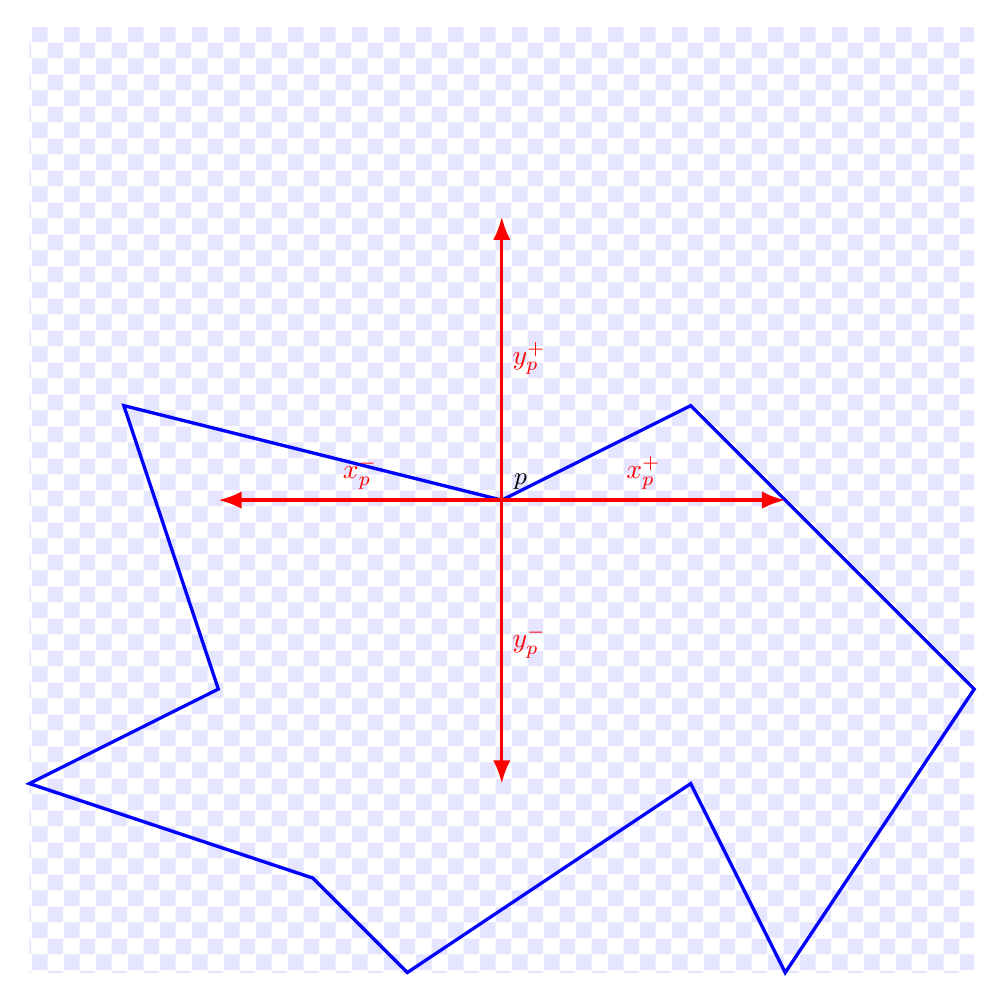
\begin{tikzpicture}[scale=1.2]
    % Background pattern
    \fill[pattern=checkerboard, pattern color=blue!20, opacity=0.5] (-5,-5) rectangle (5,5);
    
    % Irregular polygon
    \draw[blue, very thick] (0,0) -- (-4,1) -- (-3,-2) -- (-5,-3) -- (-2,-4) -- (-1,-5)
                            -- (2,-3) -- (3,-5) -- (5,-2) -- (2,1) -- cycle;
    
    % Arrows
    \draw[red, very thick, -Latex] (0,0) -- (0,3) node[midway, right] {$y_p^+$};
    \draw[red, very thick, -Latex] (0,0) -- (0,-3) node[midway, right] {$y_p^-$};
    \draw[red, very thick, -Latex] (0,0) -- (-3,0) node[midway, above] {$x_p^-$};
    \draw[red, very thick, -Latex] (0,0) -- (3,0) node[midway, above] {$x_p^+$};
    
    % Center point
    \node[font=\small] at (0.2,0.2) {$p$};
\end{tikzpicture}
\end{document}